\documentclass[aspectratio=169]{beamer}

\usetheme{default}
\usefonttheme{professionalfonts}
\setbeamertemplate{navigation symbols}{}
%\usefonttheme{serif}

\setbeamerfont{title}{series=\bfseries, size=\normalfont\Large}
\setbeamercolor{title}{fg=white}

\setbeamerfont{author}{size=\normalfont\small}
\setbeamercolor{author}{fg=white}

\setbeamerfont{frametitle}{series=\bfseries, size=\normalfont}
\setbeamercolor{frametitle}{fg=white}

\setbeamerfont{framesubtitle}{size=\normalfont\large}
\setbeamercolor{framesubtitle}{fg=white}

\setbeamercolor{background canvas}{bg=black}
\setbeamercolor{normal text}{fg=white}

\usepackage[utf8]{inputenc}
\usepackage[french]{babel}
\usepackage{amsmath}
\usepackage{amsfonts}
\usepackage{amssymb}
\usepackage{graphicx}
\usepackage[]{bm}
\usepackage[]{multimedia}

\graphicspath{{imgs/}}

\usepackage{tikz} % Required for drawing custom shapes
\usetikzlibrary{arrows}
\usetikzlibrary{shapes.geometric, math, positioning, calc, patterns, angles, quotes}
\usetikzlibrary{patterns.meta,decorations.pathmorphing}




\usepackage[]{listings}

\definecolor{codegreen}{rgb}{0,0.6,0}
\definecolor{codegray}{rgb}{0.5,0.5,0.5}
\definecolor{codepurple}{rgb}{0.58,0,0.82}
\definecolor{backcolour}{rgb}{0.0, 0.0, 0.0}

\lstdefinestyle{mystyle}{
  backgroundcolor=\color{backcolour},
  commentstyle=\color{codegreen},
  keywordstyle=\color{magenta},
  numberstyle=\tiny\color{codegray},
  stringstyle=\color{codepurple},
  basicstyle=\ttfamily\footnotesize,
  breakatwhitespace=false,
  breaklines=true,
  captionpos=b,
  keepspaces=true,
  numbers=left,
  numbersep=5pt,
  showspaces=false,
  showstringspaces=false,
  showtabs=false,
  tabsize=2
}

\lstset{style=mystyle}



\title{Introduction à Python}
\author{Jean-Christophe LOISEAU}
\institute{Arts \& Métiers Institute of Technology, 2021-2022}
\date{}

\begin{document}

\frame{\titlepage}

\begin{frame}%{Hello world}{Hello world subtitle}
  \vfill
  \begin{minipage}{.68\textwidth}
    \textbf{\alert{Python}}: langage de programmation sous licence libre créé en 1991 par \textbf{Guido van Rossum}.
  \end{minipage}%
  \hfill
  \begin{minipage}{.28\textwidth}
    \centering
    
\includegraphics[width=\textwidth]{logo_python}
  \end{minipage}
  \vfill
\end{frame}

\begin{frame}
  \vfill
  \centering
  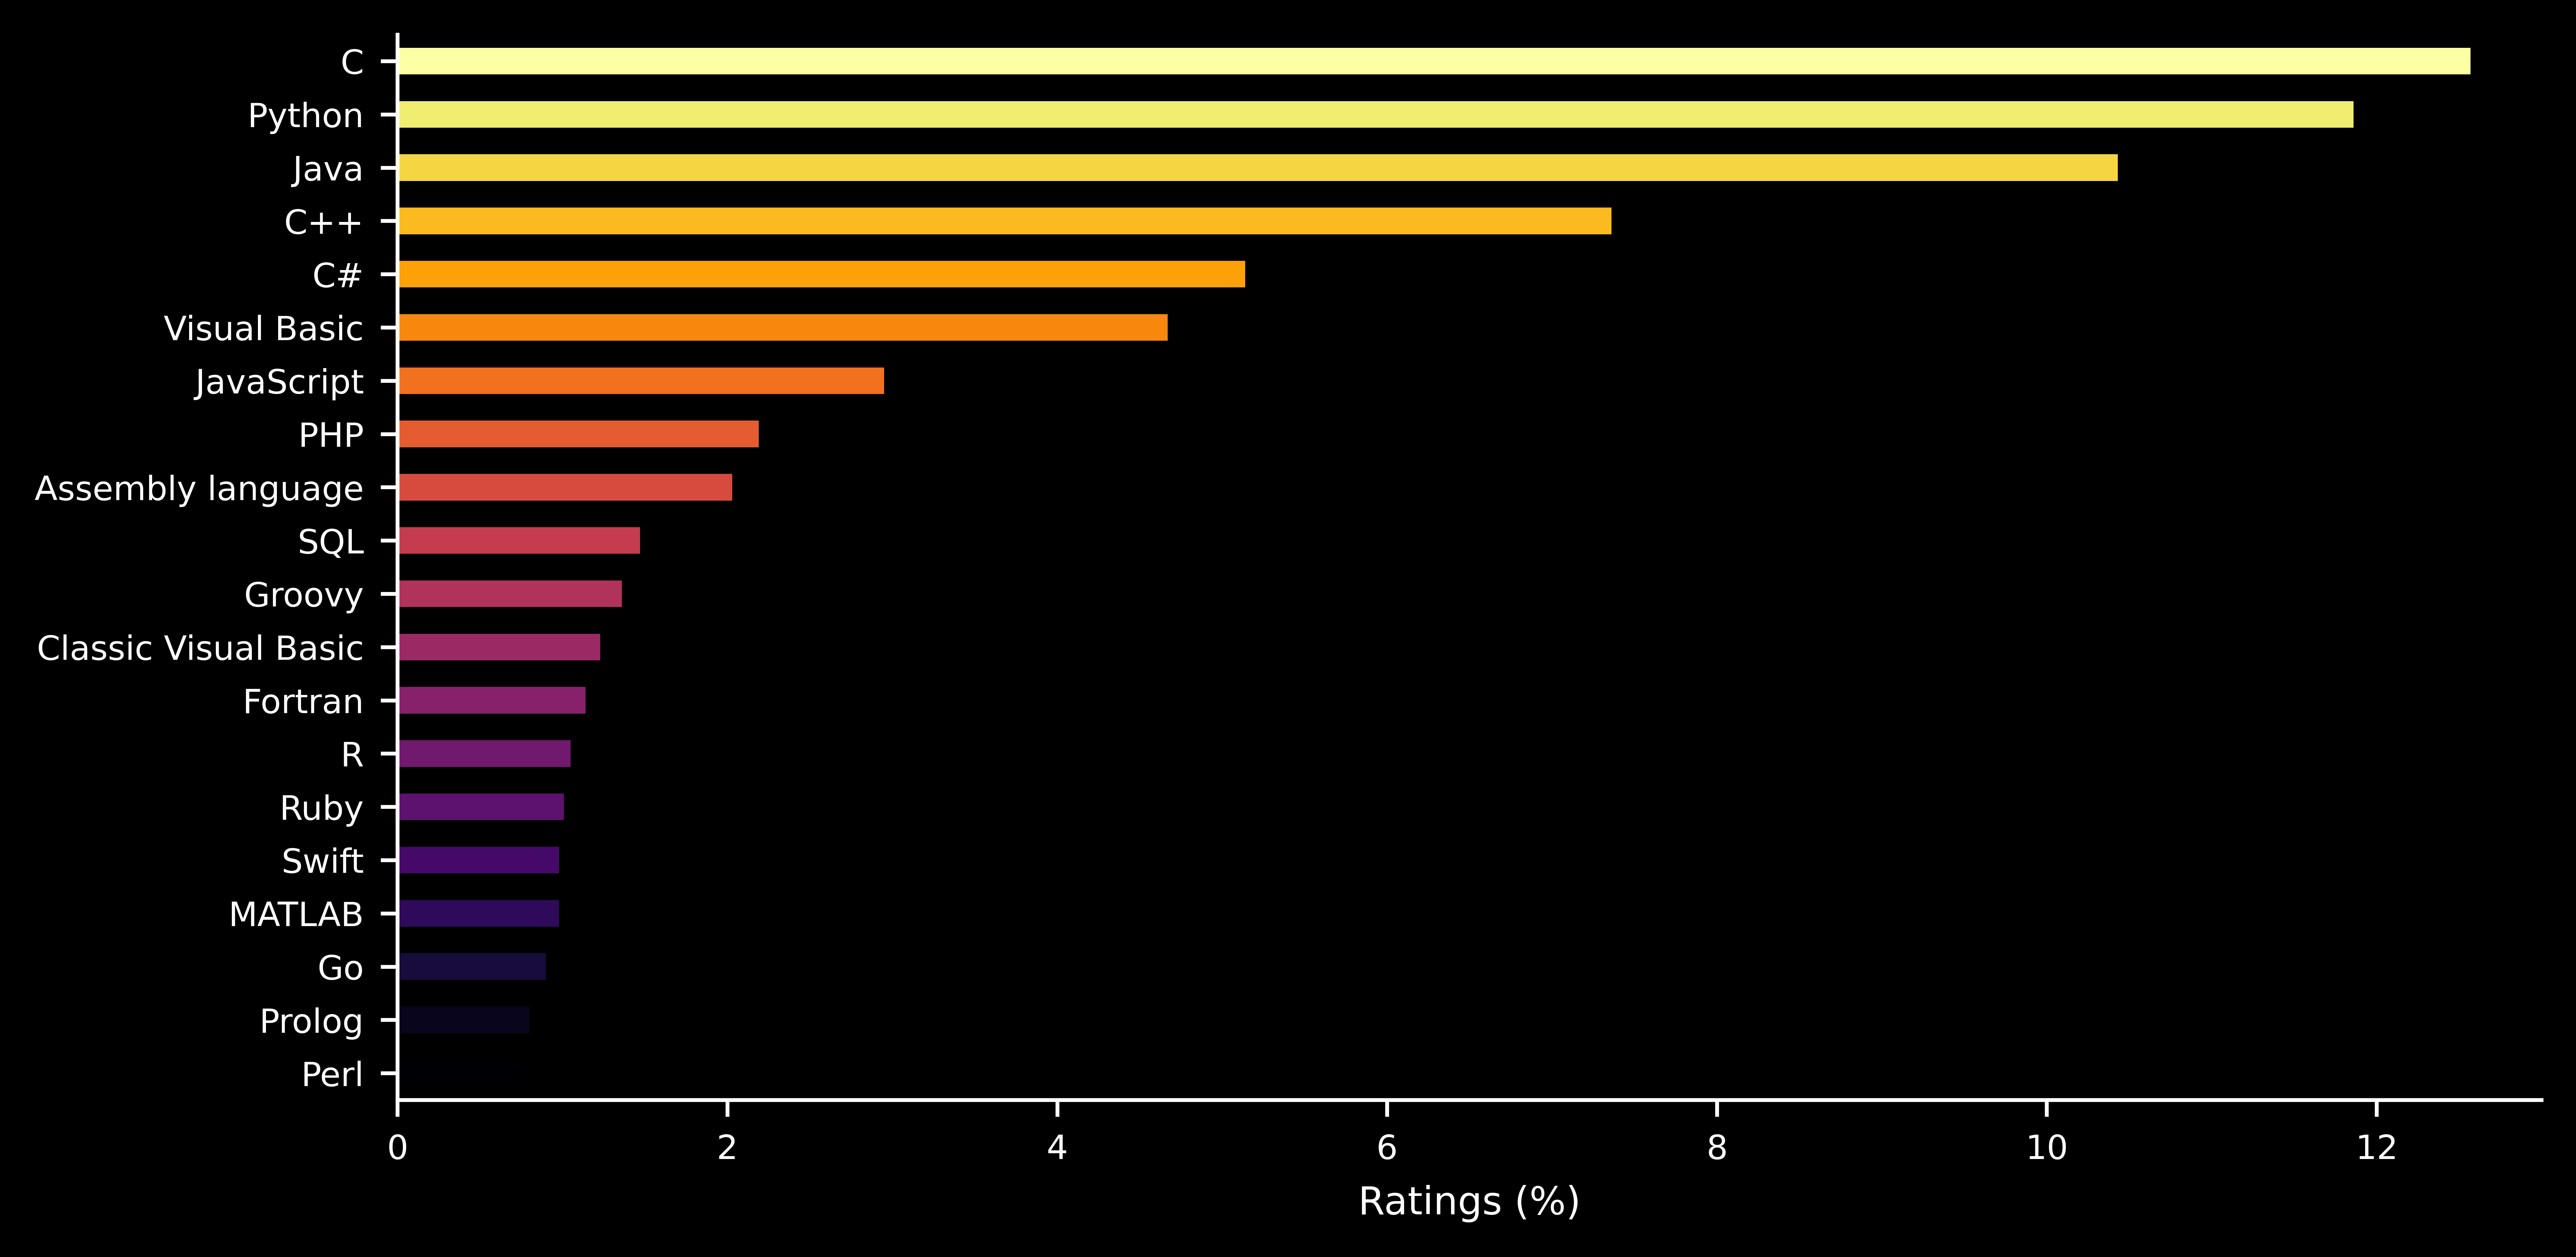
\includegraphics[width=\textwidth]{tiobe_ratings}
  \vfill
\end{frame}

\begin{frame}
\end{frame}

\begin{frame}
  \vfill
  \centering
  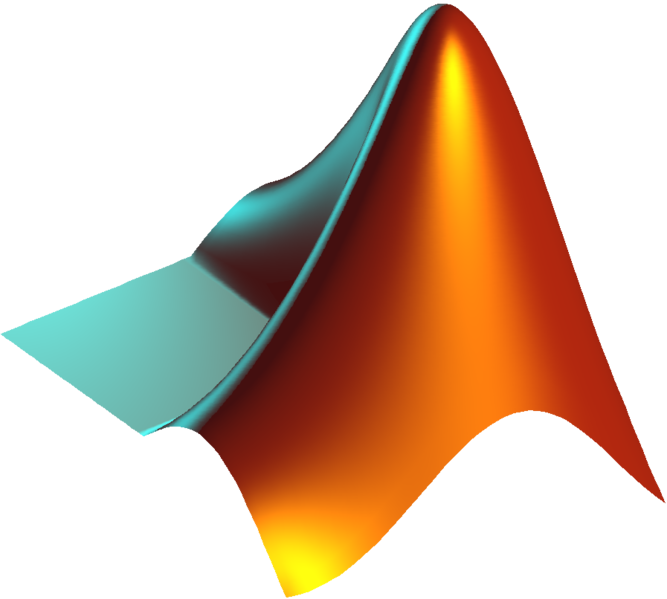
\includegraphics[width=.16\textwidth]{matlab_logo}%
  \hfill
  
\includegraphics[width=.16\textwidth]{octave_logo}%
  \hfill
  
\includegraphics[width=.16\textwidth]{fortran_logo}%
  \hfill
  
\includegraphics[width=.24\textwidth]{julia_logo}
  \vfill
\end{frame}

\begin{frame}

  \begin{minipage}{.64\textwidth}
    \textbf{\alert{NumPy}} : bibliothèque (ou package) pour \textbf{Python} destinée à manipuler des \textbf{matrices} ou \textbf{tableaux multidimensionels} ainsi que des fonctions mathématiques opérant sur ces tableaux.
  \end{minipage}%
  \hfill
  \begin{minipage}{.32\textwidth}
    \centering
    
\includegraphics[width=\textwidth]{numpy_logo}
  \end{minipage}

  \vspace{-1cm}
\end{frame}

\begin{frame}

  \begin{minipage}{.64\textwidth}
    \textbf{\alert{SciPy}} : NumPy sous stéroïdes permettant de faire de l'optimisation, algèbre linéaire, statistiques, traitement du signal ou d'images, intégration numérique et simulation.
  \end{minipage}%
  \hfill
  \begin{minipage}{.32\textwidth}
    \centering
    
\includegraphics[width=.75\textwidth]{scipy_logo}
  \end{minipage}

  \vspace{-1cm}
\end{frame}

\begin{frame}

  \begin{minipage}{.64\textwidth}
    \textbf{\alert{Matplotlib}} : Package Python pour tracer et visualiser des données sous formes de graphiques ou d'animations.
  \end{minipage}%
  \hfill
  \begin{minipage}{.32\textwidth}
    \centering
    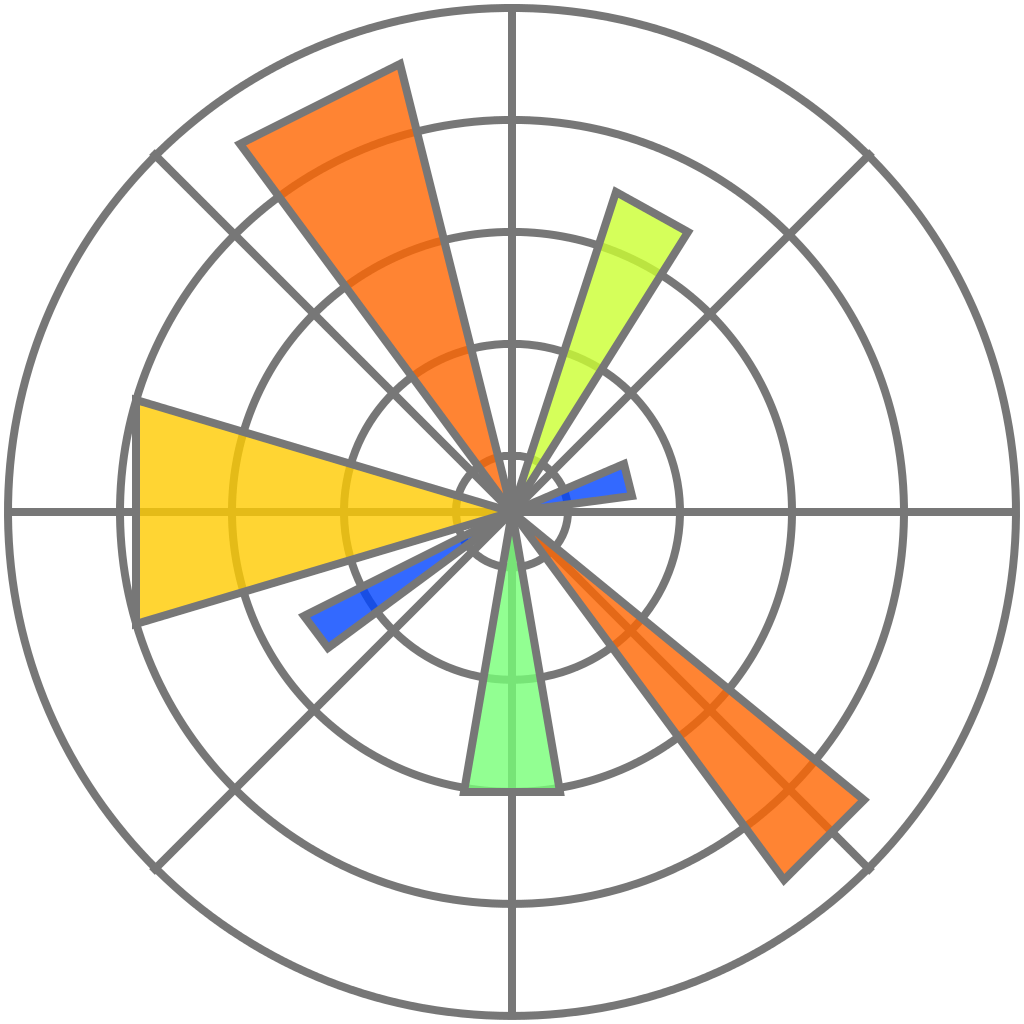
\includegraphics[width=.75\textwidth]{matplotlib_logo}
  \end{minipage}

  \vspace{-1cm}
\end{frame}

\begin{frame}
  \vfill
  \centering
  \textbf{Quelques exemples d'applications}
  \vfill
\end{frame}

\begin{frame}[t, c]{Mécanique}{}
  \vfill

  \begin{minipage}{.48\textwidth}
    \centering
    \textbf{Mécanique Lagrangienne}

    \[
    \mathcal{L}(x, \dot{x}) = E_c - E_p \]
    \[
    \dfrac{d}{dt} \left( \dfrac{\partial \mathcal{L}}{\partial \dot{x}} \right) - \dfrac{\partial \mathcal{L}}{\partial x} = F
    \]
  \end{minipage}%
  \hfill
  \begin{minipage}{.48\textwidth}
      \begin{tikzpicture}[>=stealth]
      \path[pattern={Lines[angle=45,distance={8pt/sqrt(2)}]}] (-2, 5) edge ++(4,0) rectangle ++ (4, 0.5);

      \draw[decorate,decoration={coil, segment length=5pt, aspect=0.7, amplitude=4pt,
          pre=lineto, pre length=5mm, post=lineto, post length=5mm}] (0.5, 5) -- (0.5, 2.5)
      node[left, draw, minimum size=1cm, fill=gray] (m) {$m$};

      \draw[] (-0.5, 5) -- (-0.5, 4) {};
      \draw[] (-0.25, 4) -- (-0.75, 4) {};

      \draw[] (-0.5, 3.75) -- (-0.5, 2.5) {};
      \draw[] (-0.25, 3.75) -- (-0.75, 3.75) {};

      \draw[] (-0.25, 3.75) -- (-0.25, 4.25) {};
      \draw[] (-0.75, 3.75) -- (-0.75, 4.25) {};

      \draw[red] (m.center-|0, 0) ++ (0, 1) -- ++ (-2, 0)
      edge[<-,edge label'=$x$,shorten >=1pt] (m.center-|-2, 0)
      (m.center-|0, 0) ++ (0, -1) -- ++ (-2, 0) 
      edge[<-,edge label=$-x$,shorten >=1pt] (m.center-|-2, 0)
      (m.east) edge[dashed] (m.east-|2, 0) 
      (m.east-|2, 0) node[right] {Equilibrium};
  \end{tikzpicture}

  \end{minipage}

  \vfill
\end{frame}

\begin{frame}[fragile]{}{}
  \vfill
  \begin{lstlisting}[language=Python]
    import numpy as np
    from scipy.integrate import solve_ivp
    
    def eom(t, u, k):
        # --> Degres de liberte.
        x, dx = u
        # --> Eq. du mvt.
        ddx = -x - 2*k*dx
        return dx, ddx
    
    # --> Parametres de la simulation.
    u = np.array([1.0, 0.0])
    k = 0.05
    tspan = (0.0, 100.0)
    
    # --> Simulation
    output = solve_ivp(
        lambda t, u : eom(t, u, k),
        tspan,
        u)
  \end{lstlisting}
  \vfill
\end{frame}

\begin{frame}[t, c]{Epidémiologie}{}
  \vfill
  \begin{minipage}{.28\textwidth}
    \[
    \begin{aligned}
      \dfrac{dS}{dt} & = - R_0 SI \\
      \dfrac{dI}{dt} & = R_0 SI - I \\
      \dfrac{dR}{dt} & = I
    \end{aligned}
    \]
  \end{minipage}%
  \hfill
  \begin{minipage}{.68\textwidth}
    \textbf{SIR} : Modèle classique utilisé en épidémiologie depuis les années 1930.
    Forme actuellement la base des modèles pour prédire l'évolution de COVID 19.
  \end{minipage}
  \vfill
\end{frame}

\begin{frame}
  \centering
  \vfill
  \movie[width=\textwidth, autostart, loop]{
    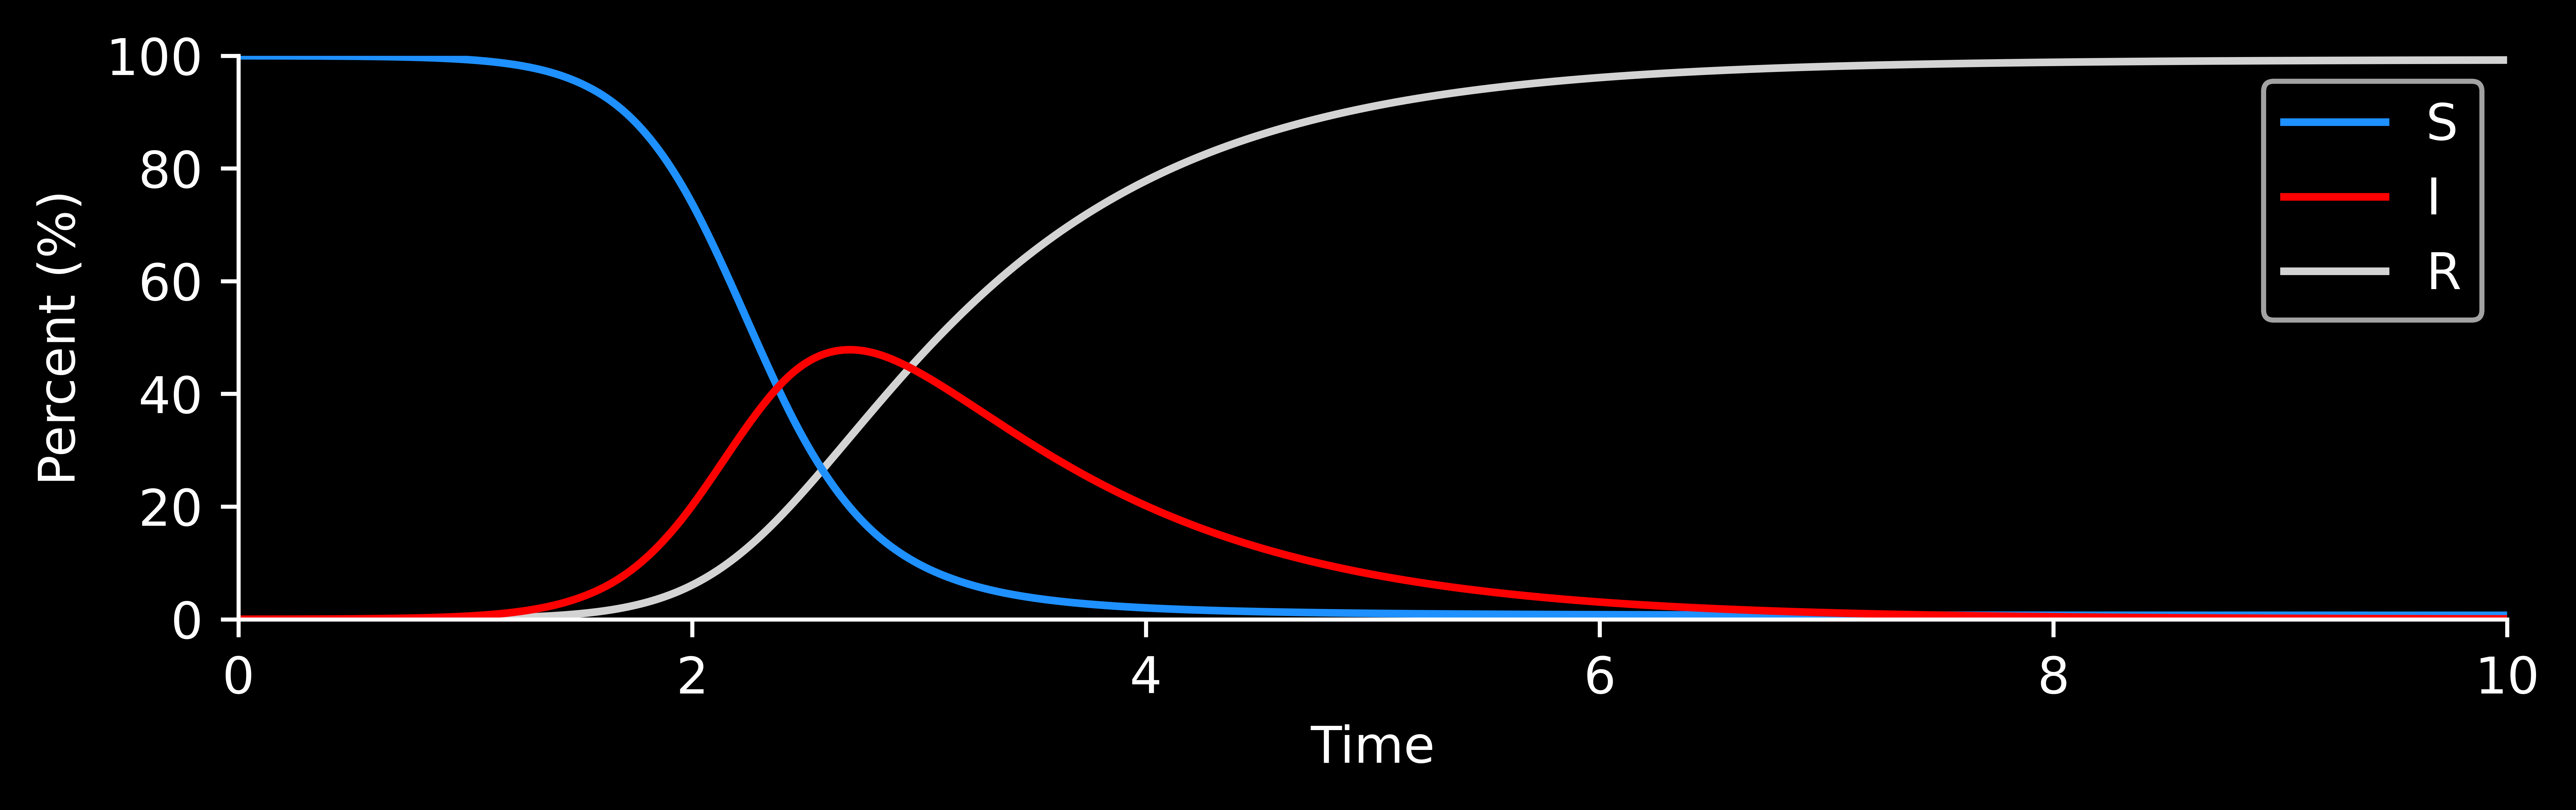
\includegraphics[width=\textwidth]{sir_final}
  }{imgs/sir_model.mp4}
  \vspace{-1cm}
  \vfill
\end{frame}

\begin{frame}[t, c]{Hydraulique}{}
  \vfill
  \begin{minipage}{.48\textwidth}
    \[
    \dfrac{1}{\sqrt{f_D}} = -2 \log_{10} \left( \dfrac{\epsilon}{3.7D} + \dfrac{2.51}{Re \sqrt{f_D}} \right)
    \]
  \end{minipage}%
  \hfill
  \begin{minipage}{.48\textwidth}
    \centering
    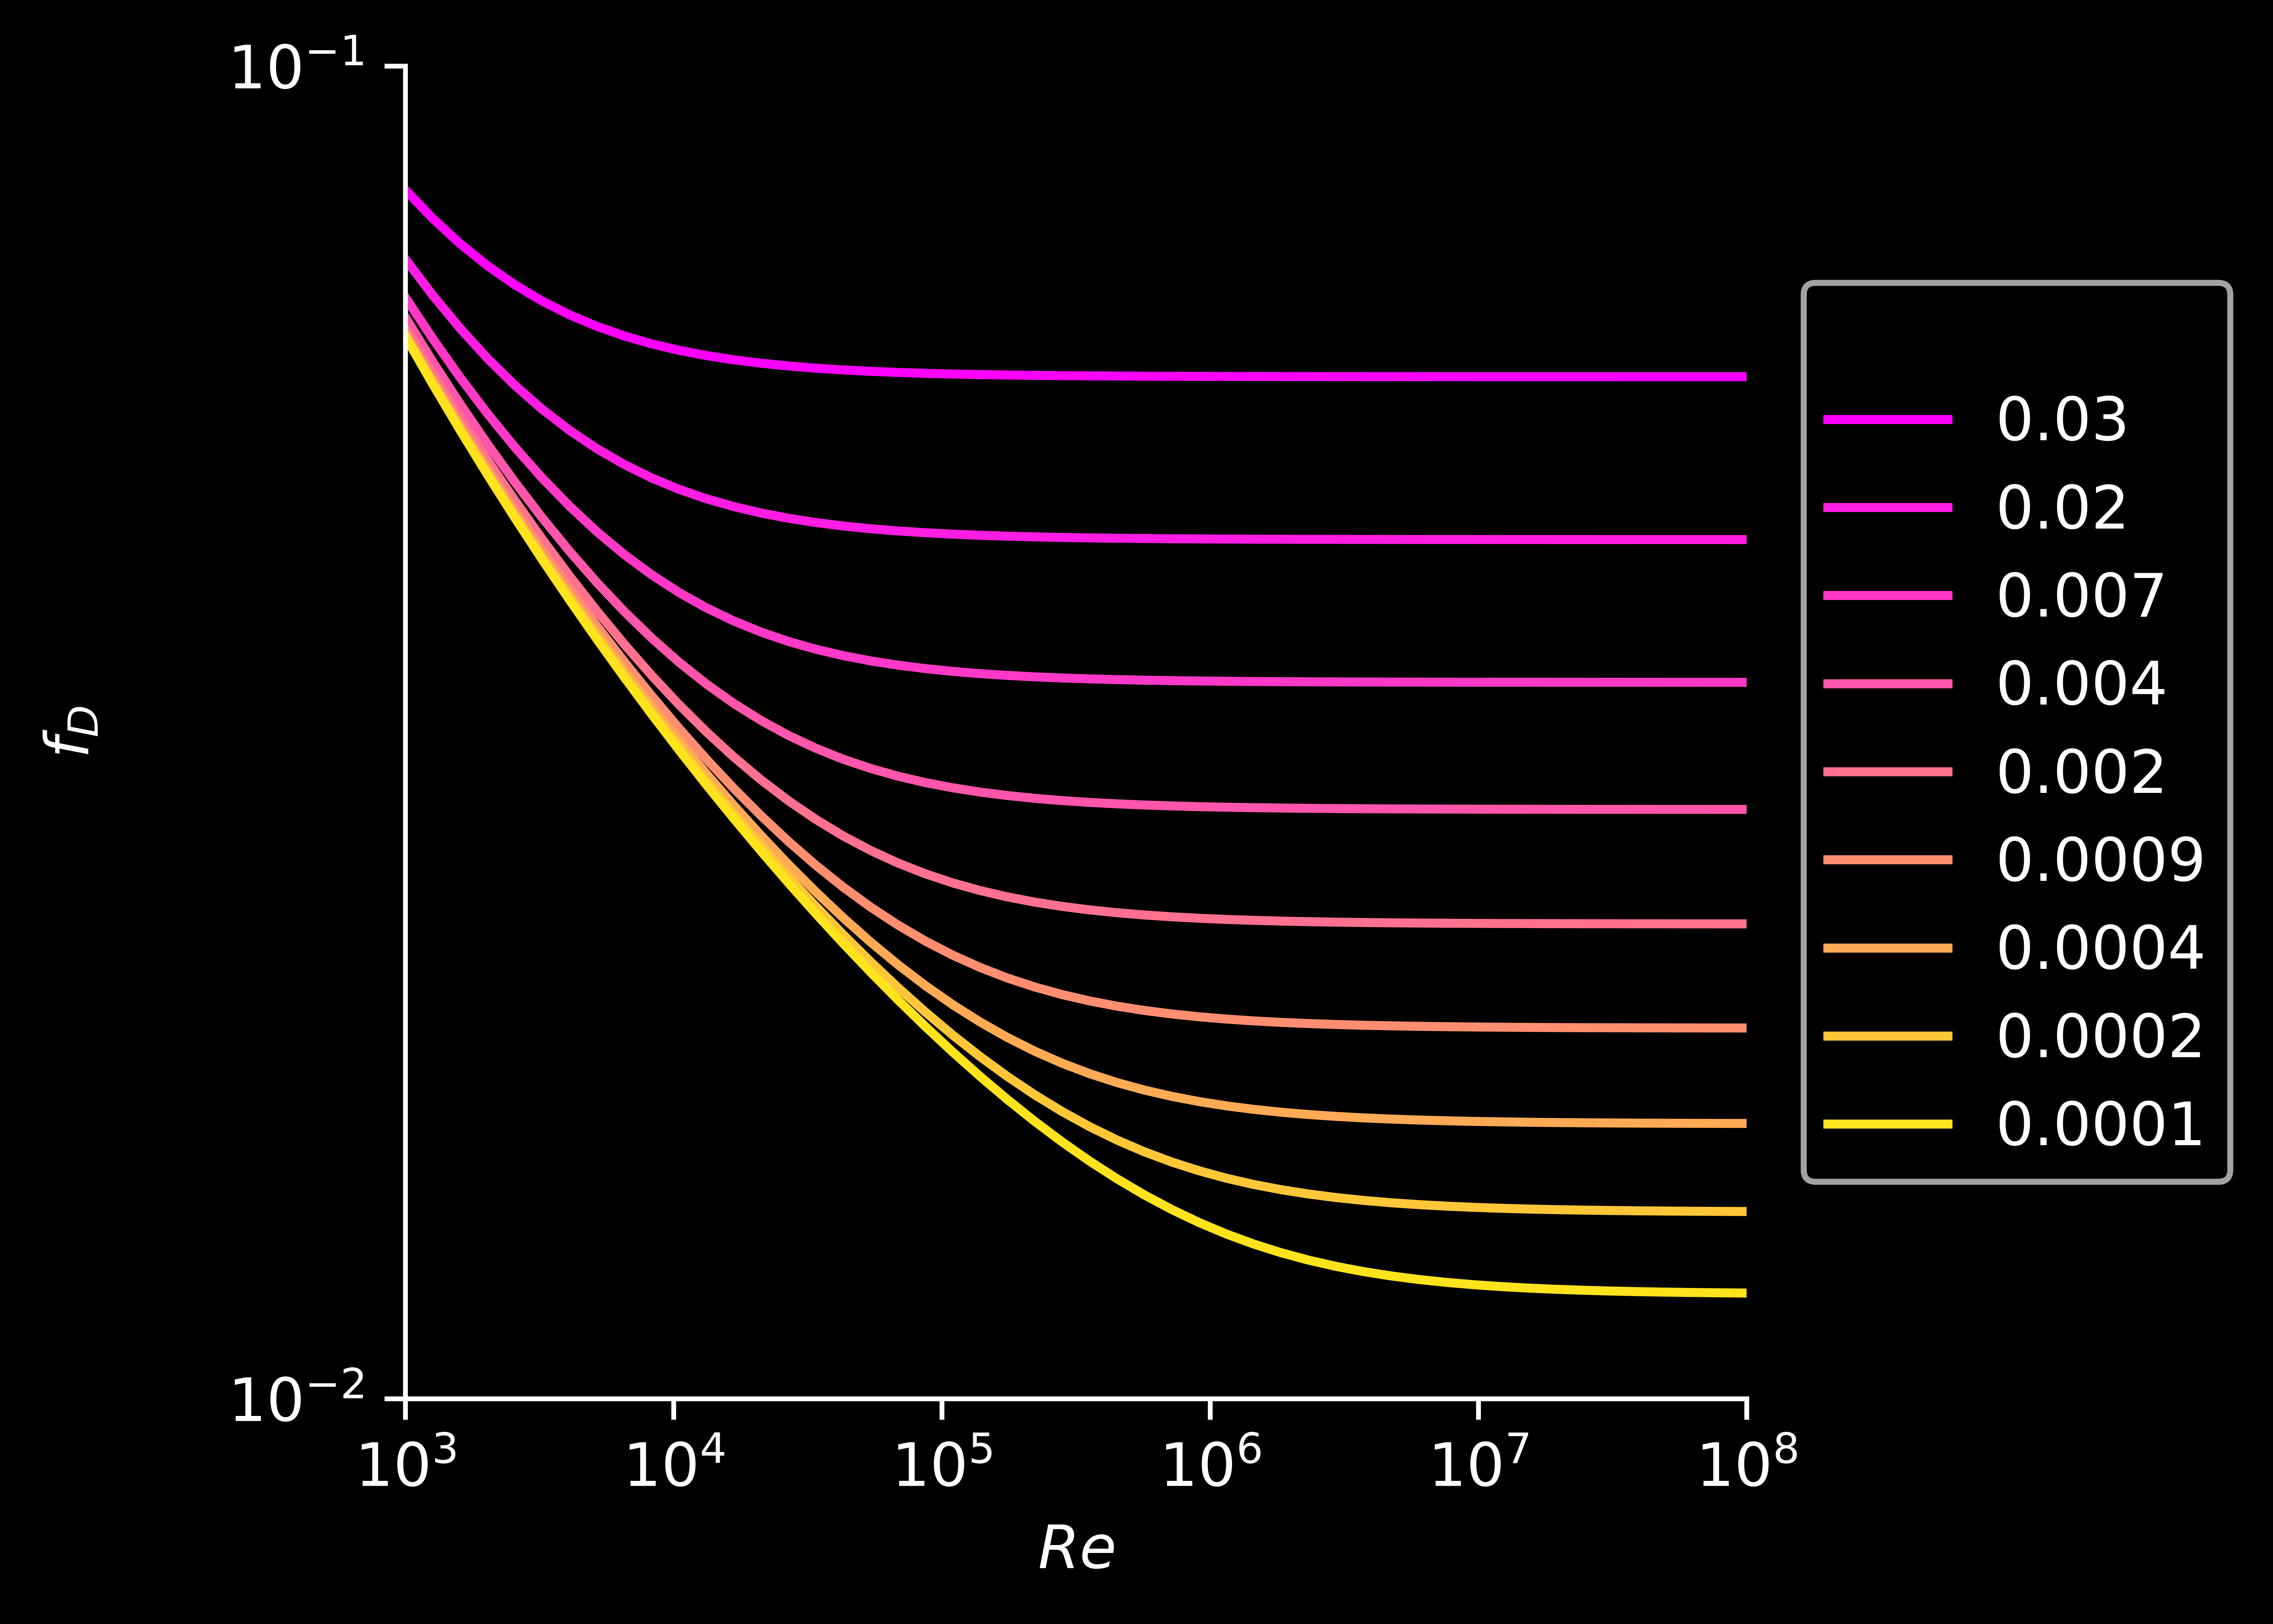
\includegraphics[width=\textwidth]{moody_chart}
  \end{minipage}
  \vfill
\end{frame}

\begin{frame}[t, c]{Dynamique des fluides}{}
  \begin{minipage}{.48\textwidth}
    \[
    \begin{aligned}
      \dfrac{\partial \bm{u}}{\partial t} + \nabla \cdot \left( \bm{u} \otimes \bm{u} \right) & = -\nabla p + \dfrac{1}{Re} \nabla^2 \bm{u} \\
      \nabla \cdot \bm{u} & = 0
    \end{aligned}
    \]
  \end{minipage}%
  \hfill
  \begin{minipage}{.48\textwidth}
    \centering
    \movie[width=\textwidth, autostart, loop]{
      
\includegraphics[width=\textwidth]{2D_turbulence}
    }{imgs/2D_turbulence.mp4}
  \end{minipage}
\end{frame}

\begin{frame}[t, c]{Traitement de l'image}{}
  \begin{overprint}
    \onslide<1>
    \vfill
    \centering
    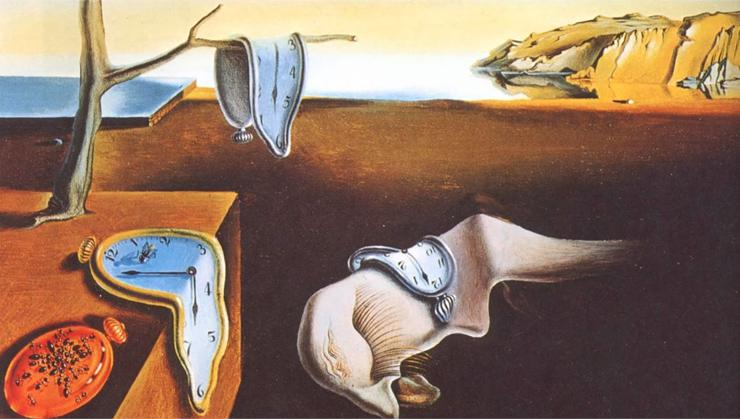
\includegraphics[height=.75\textheight]{raw_img}
    \vfill

    \onslide<2>
    \vfill
    \centering
    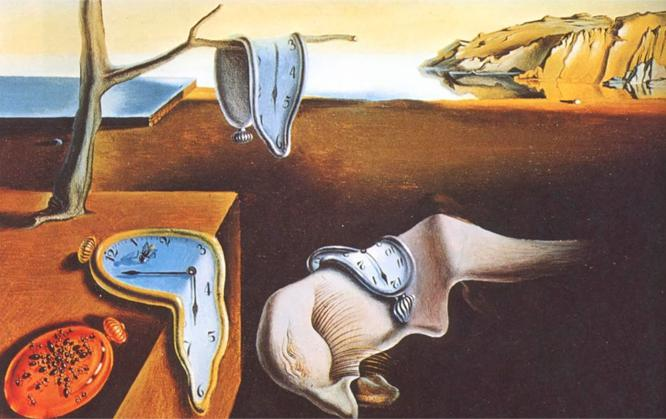
\includegraphics[height=.75\textheight]{cropped_img_0004}
    \vfill

    \onslide<3>
    \vfill
    \centering
    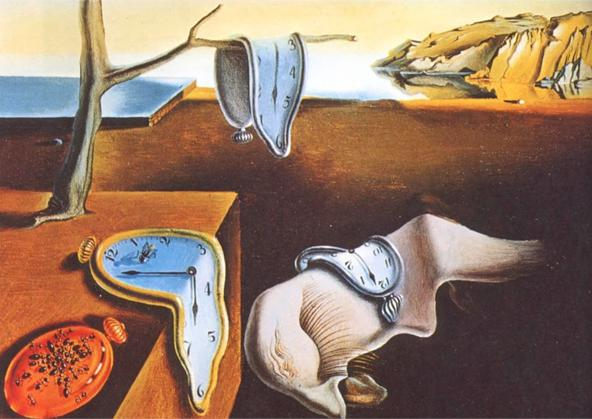
\includegraphics[height=.75\textheight]{cropped_img_0003}
    \vfill

    \onslide<4>
    \vfill
    \centering
    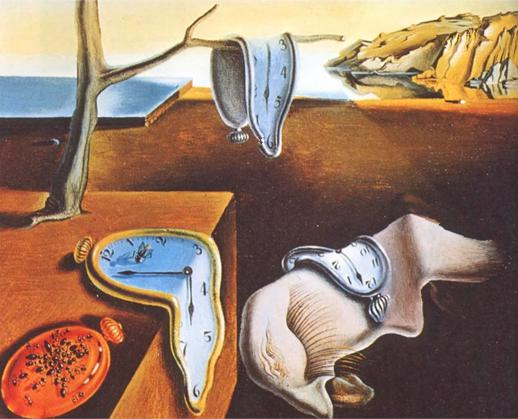
\includegraphics[height=.75\textheight]{cropped_img_0002}
    \vfill

    \onslide<5>
    \vfill
    \centering
    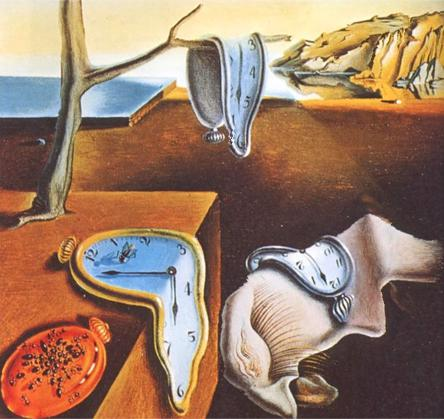
\includegraphics[height=.75\textheight]{cropped_img_0001}
    \vfill

    \onslide<6>
    \vfill
    \centering
    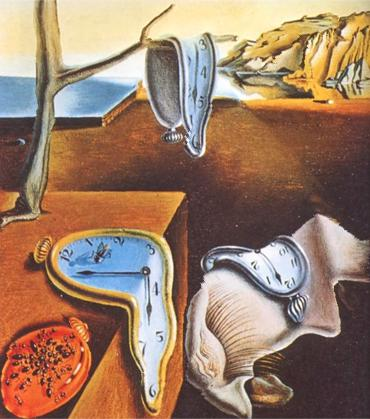
\includegraphics[height=.75\textheight]{cropped_img_0000}
    \vfill

  \end{overprint}
\end{frame}

\begin{frame}[t, c]{Machine Learning}{}
  \vfill
  \centering
  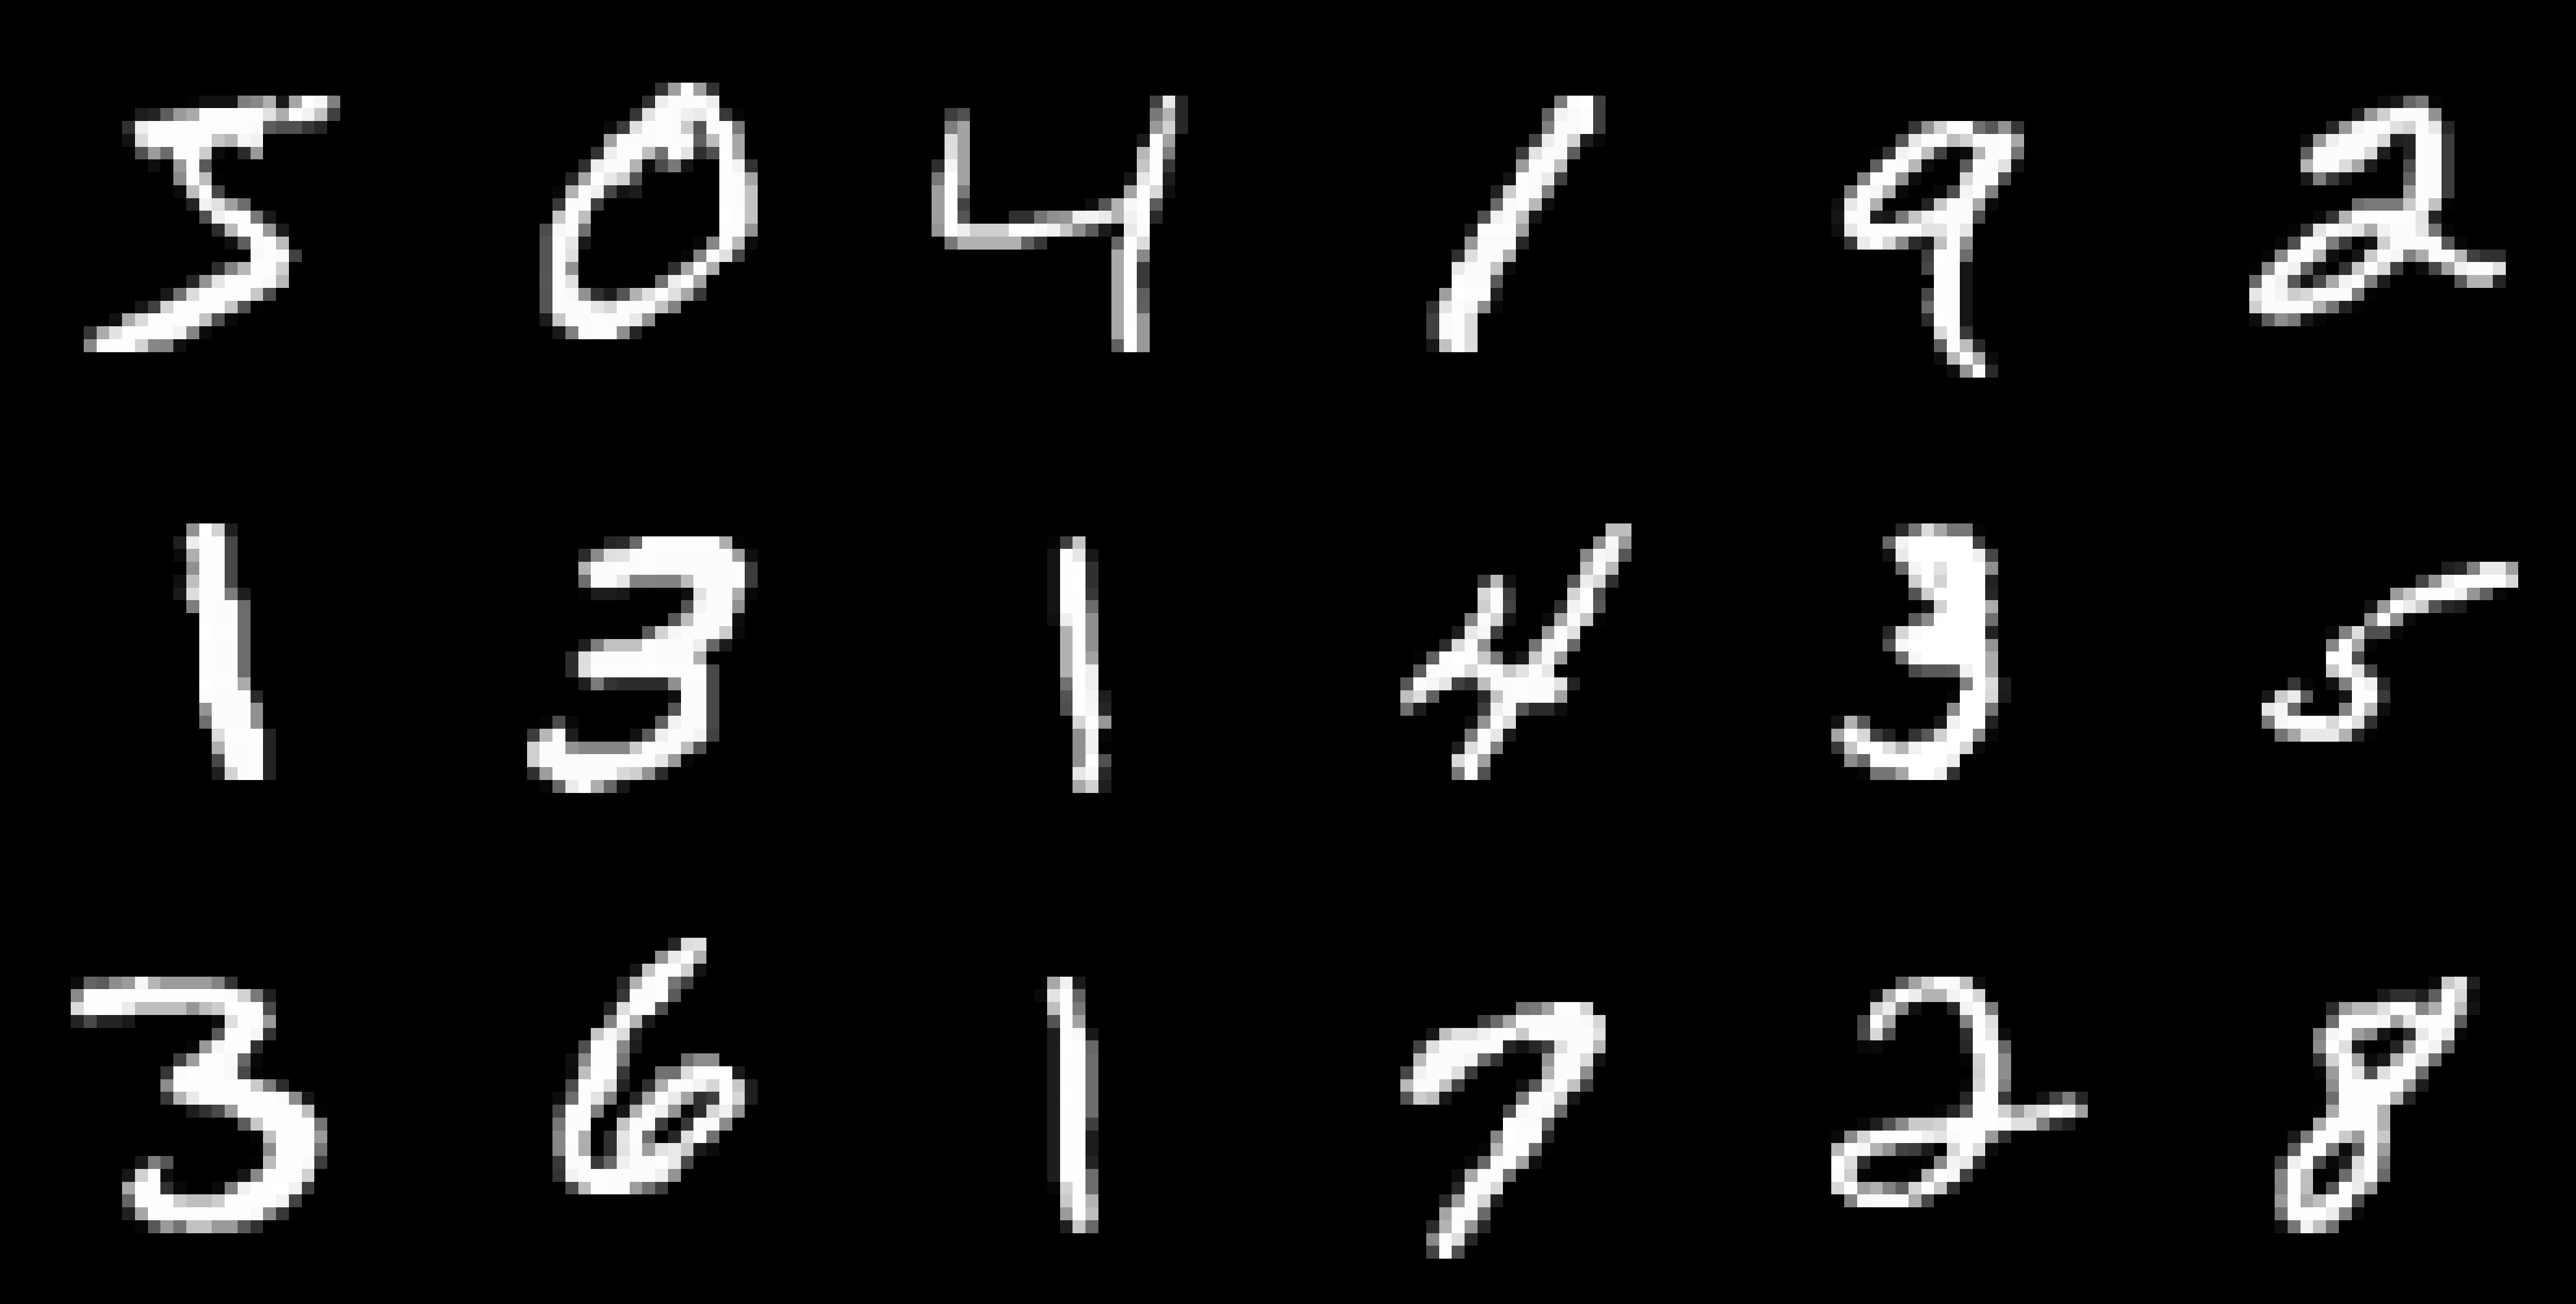
\includegraphics[width=\textwidth]{mnist_examples}
  \vfill
\end{frame}

\begin{frame}[t, c]{Machine Learning}{}
  \vfill
  \begin{minipage}{.48\textwidth}
    \centering

    Modèle : \( y_i = f(\bm{x}_i, \boldsymbol{\theta}) \)

    \[
    \textrm{minimize} \quad \sum_{i=1}^N \mathcal{J}(y_i, \hat{y}_i)
    \]
  \end{minipage}%
  \hfill
  \begin{minipage}{.48\textwidth}
    \centering
    \movie[width=\textwidth, autostart, loop]{
      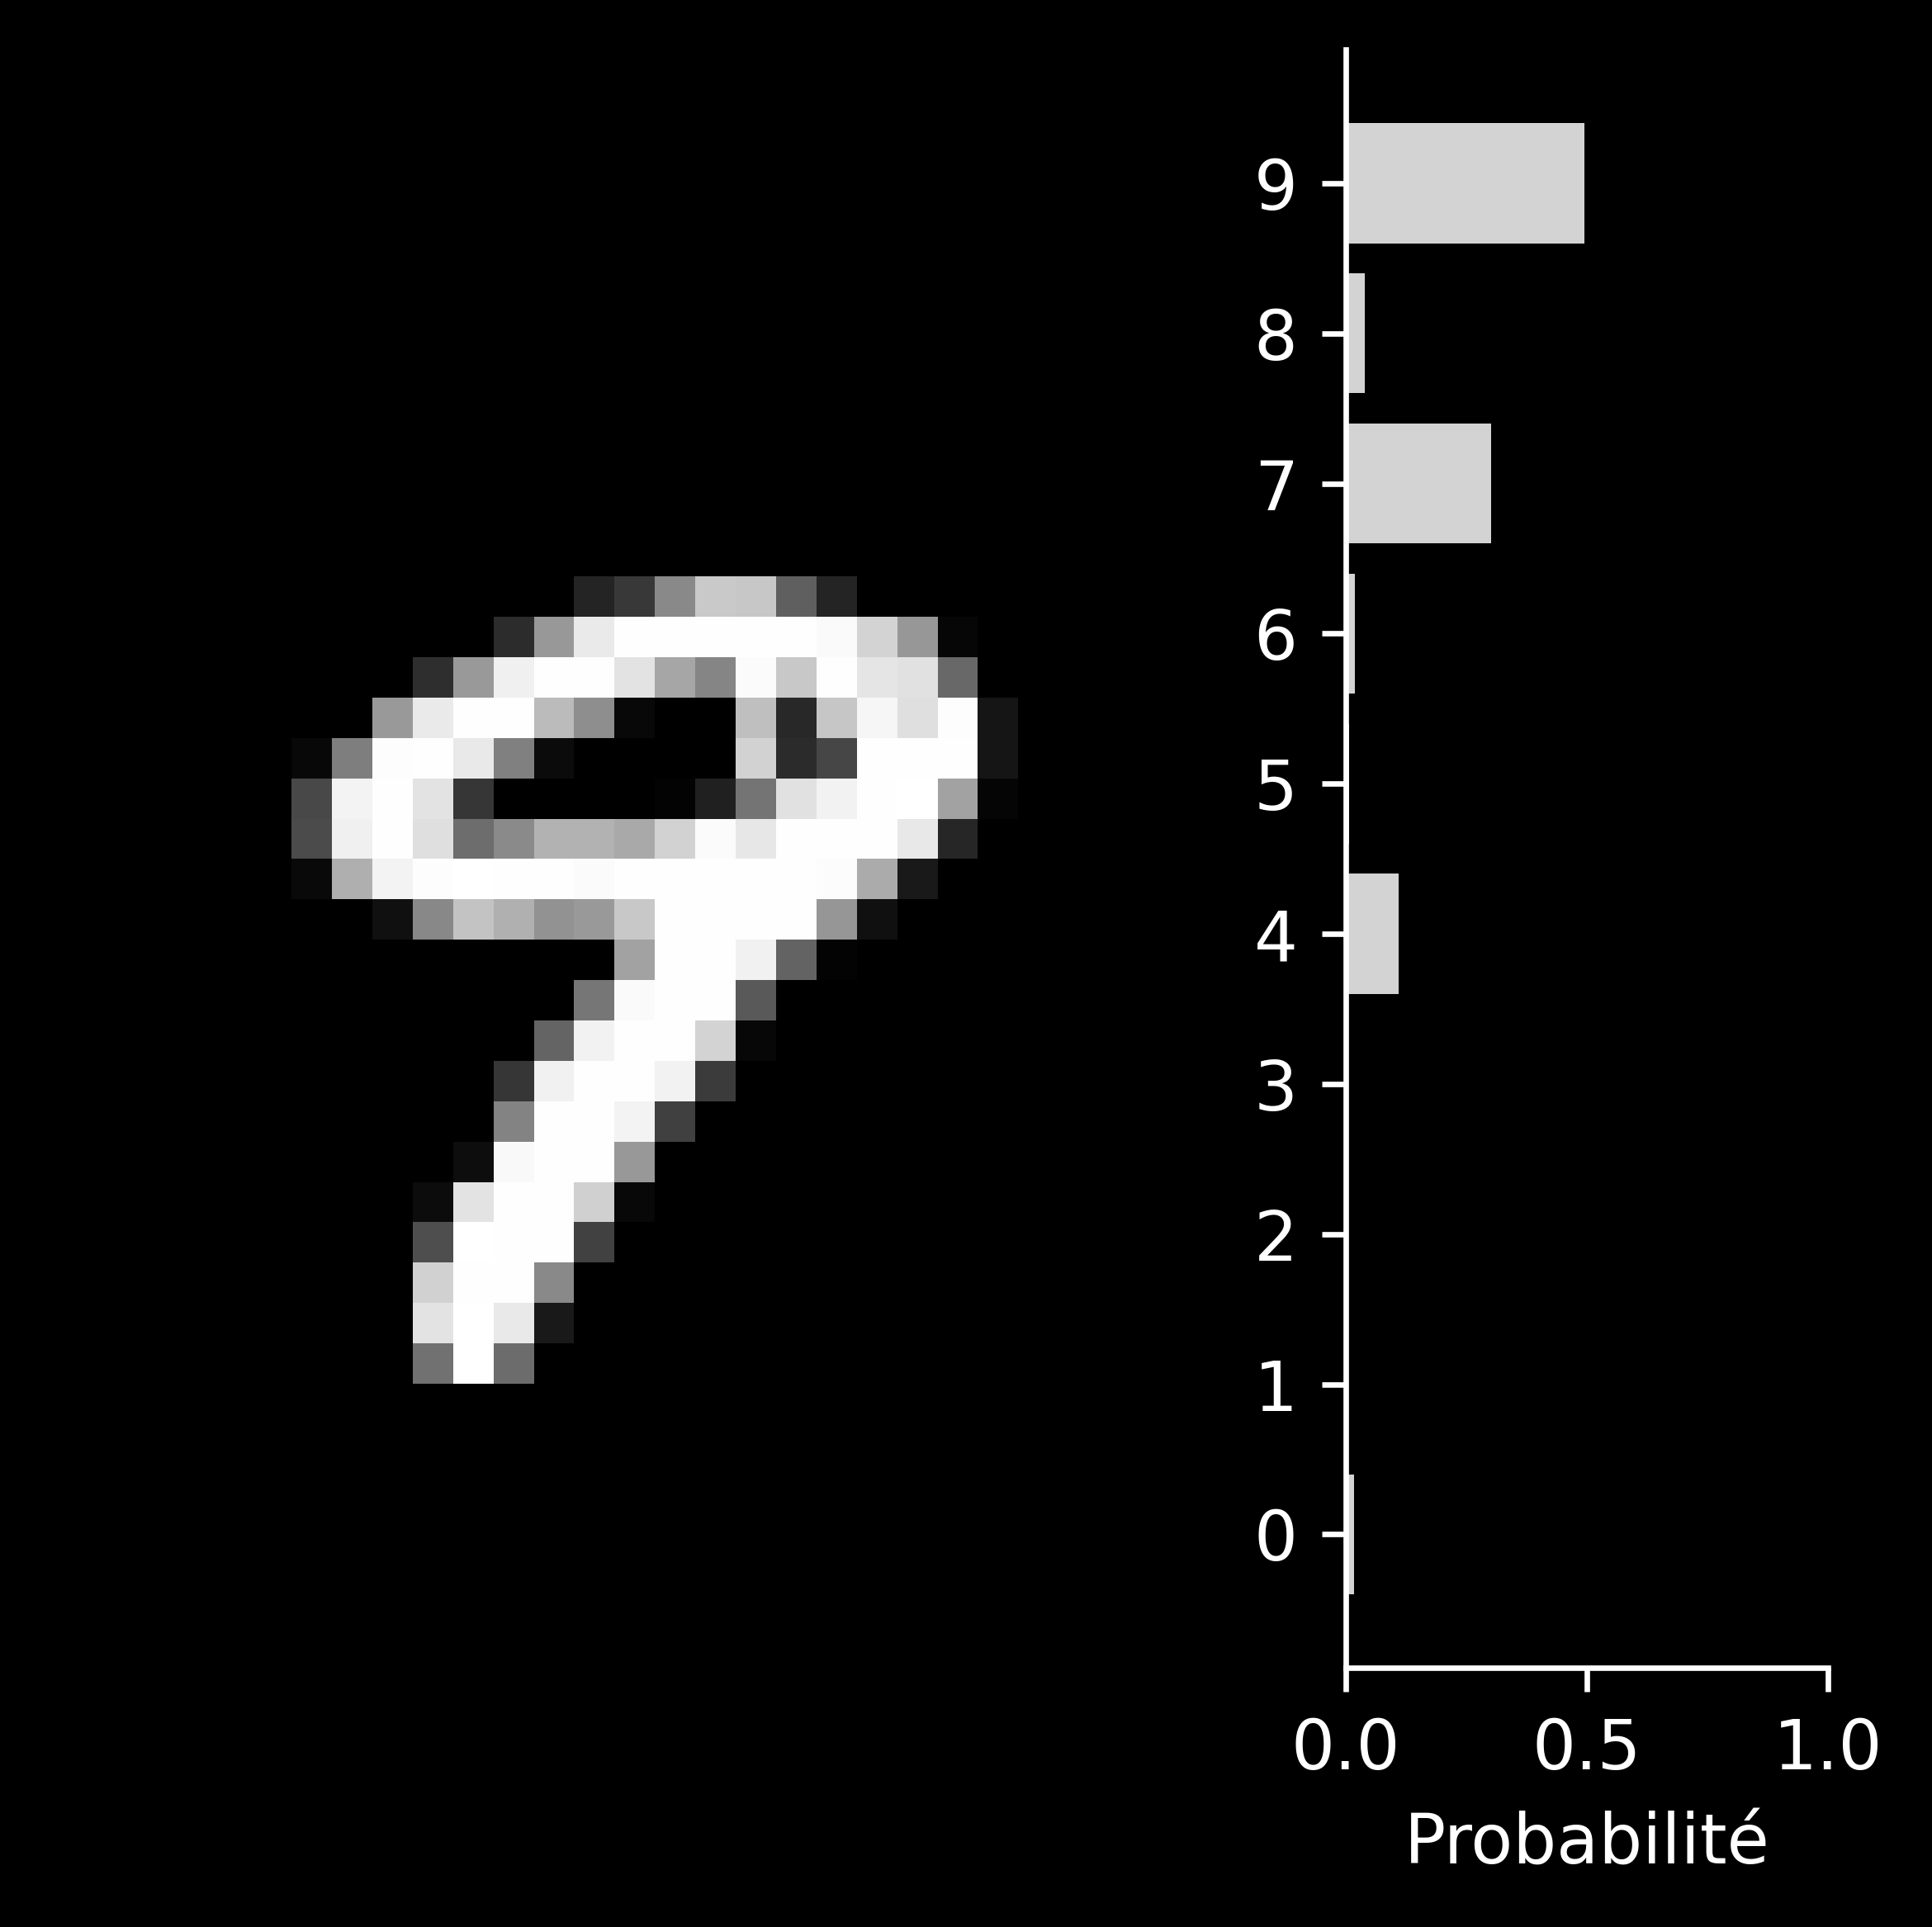
\includegraphics[width=\textwidth]{mnist_one_digit}
    }{imgs/mnist_one_digit.mp4}
  \end{minipage}
  \vfill
\end{frame}

\begin{frame}
\end{frame}

\end{document}
